%%This is a very basic article template.
%%There is just one section and two subsections.
\documentclass{beamer}

\usepackage[brazilian]{babel}%
\usepackage[utf8]{inputenc}%
\usepackage{lmodern}%
\usepackage{transparent}
\usepackage{xcolor}

\usepackage{tcolorbox}
\DeclareOptionBeamer{compress}{\beamer@compresstrue}
\ProcessOptionsBeamer

\mode<presentation>

\useoutertheme[footline=authortitle]{miniframes}
\useinnertheme{circles}
\usecolortheme{whale} 
\usecolortheme{orchid}

\definecolor{beamer@blendedblue}{rgb}{0.137,0.466,0.741}

\setbeamercolor{structure}{fg=beamer@blendedblue}
\setbeamercolor{titlelike}{parent=structure}
\setbeamercolor{frametitle}{fg=black}
\setbeamercolor{title}{fg=black}
\setbeamercolor{item}{fg=black}

\mode 
<all>
 
\title[]{Controle de estabilidade veicular com MPC baseado em modelo LTI com
perturbação e restrições utilizando parametrização}% \subtitle{Exemplo
% Funcional}%
\author{ Zoé Magalhães \\%
         \texttt{zoe.magalhaes@unb.br}}%
\institute[PPMEC]{Departamento de Engenharia Mecânica\\%
                Universidade de Brasília}%
\date[2018]{}%


%% Formata um comando.
\makeatletter%
\newcommand{\comm}[2][]{% 
    \texttt{{\textbackslash}#2}%
    \if#1\@empty% 
    \else\{#1\}\fi%
}%
\makeatother

\begin{document} 

\frame{\titlepage}%x`

\section{Objetivo}%
  
\begin{frame}[t]% s
	\begin{itemize}
		\item Objetivo 
	\end{itemize}
	Controlador que calcule o momento de guinada externo necessário para:
	\begin{itemize}
	  \item corrigir o deslizamento lateral
	  \item corrigir o erro na taxa de guinada
	\end{itemize}
	  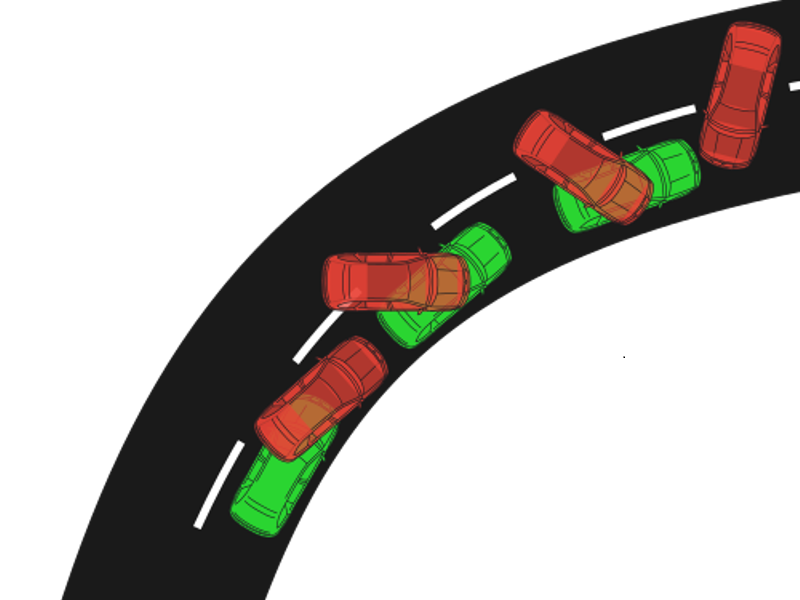
\includegraphics[width=0.6\textwidth]{oversteer.png}%
\end{frame}
  
%%%%%%%%%%%%%%%%%%%%%%%%%%%%%%%%%%%%%%%%%%%%%%%%%%%%%%%%%%%%%%%%%%%%%%%%
\section{Modelo}%
 \begin{frame}[t]%

            
 \begin{columns}%
      \column{.50\textwidth}%]
      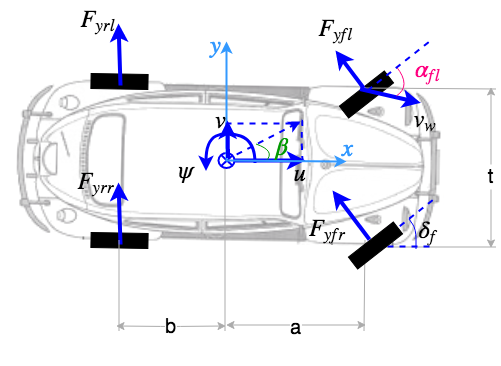
\includegraphics[width=1\textwidth]{carmodel.png}%
      \column{.50\textwidth}%
      \small
 \noindent\textbf{Movimento lateral:}
 \vspace{-0.2 cm}
    \begin{equation*}    
    \begin{split}
       	mu\left(\dot{\beta} + \dot{\psi} \right) -m_sh_s\ddot{\phi} =
       	\sum{F_y}
       	\\
    \end{split}
    \end{equation*}
\vspace{-0.2 cm}
\noindent\textbf{Guinada:} 
\vspace{-0.2 cm}
    \begin{equation*}  
    \begin{split}
       I_{zz}\ddot{\psi} - I_{xz}\ddot{\phi} &= a(F_{yfl} + F_{yfr}) \\
       &- b(F_{yrl} + F_{rr}) + M_u \\
    \end{split}
    \end{equation*}
\vspace{-0.2 cm}
\noindent\textbf{Rolagem:}
\vspace{-0.2}
\begin{equation*}
\begin{split}
	I_{xx}\ddot{\phi} - I_{xz}\ddot{\psi} & =  m_sh_su(\dot{\beta} + \dot{\psi}) \\
	& + m_sh_sg\sin(\phi) - (k_{\phi f} + k_{\phi r} ) \phi \\ 
	& - ( c_{\phi f} + c_{\phi r} ) \dot{\phi} \\
 \end{split}        
\end{equation*} 
\vspace{-0.2 cm}
    \end{columns}%
\end{frame}%

 \begin{frame}[t]%
            
 \begin{columns}%
      \column{.50\textwidth}%]
      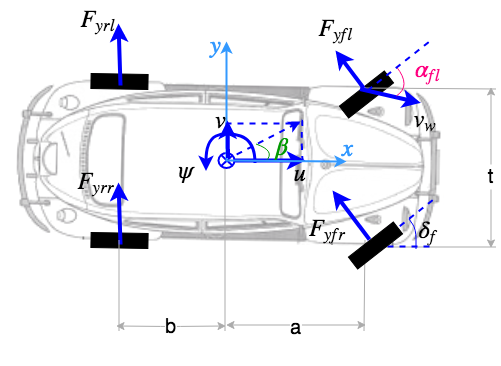
\includegraphics[width=1\textwidth]{carmodel.png}%
      \column{.50\textwidth}%
      \small
 \noindent\textbf{Movimento lateral:}
 \vspace{-0.2 cm}
    \begin{equation*}    
    \begin{split}
       	mu\left(\dot{\beta} + \dot{\psi} \right) -m_sh_s\ddot{\phi} =
       	\sum{F_y}
       	\\
    \end{split}
    \end{equation*}
\vspace{-0.2 cm}
\noindent\textbf{Guinada:} 
\vspace{-0.2 cm}
    \begin{equation*}  
    \begin{split}
       I_{zz}\ddot{\psi} - I_{xz}\ddot{\phi} &= a(F_{yfl} + F_{yfr}) \\
       &- b(F_{yrl} + F_{rr}) + M_u \\
    \end{split}
    \end{equation*}
\vspace{-0.2 cm}
\noindent\textbf{Rolagem ($\phi < \pi/16 rad$):}
\begin{equation*}
\begin{split}
	I_{xx}\ddot{\phi} - I_{xz}\ddot{\psi} & =  m_sh_su(\dot{\beta} + \dot{\psi}) \\
	& + m_sh_sg\phi - (k_{\phi f} + k_{\phi r} ) \phi \\ 
	& - ( c_{\phi f} + c_{\phi r} ) \dot{\phi} \\
 \end{split}        
\end{equation*} 
\vspace{-0.2 cm}
    \end{columns}%
\end{frame}%

%%%%%%%%%%%%%%%%%%%%%%%%%%%%%%%%%%%%%%%%%%%%%%%%%%%%%%%%%%%%%%%%%%%%%%%%
 \begin{frame}[t]%

 \noindent\textbf{Força lateral das rodas(linearização):}
    \begin{equation*}
    \begin{split}
	F_{yfi} = C_f\alpha_f \enskip&\enskip F_{yri} = C_r\alpha_r\\
    \end{split}
    \end{equation*}
\vspace{-0.2 cm}
\noindent\textbf{Deslizamento das rodas(linearização):} 
    \begin{equation*}
    \begin{split}
		\alpha_f  = -\beta - \frac{a\dot{\psi}}{u} + \delta_f \enskip&\enskip
		\alpha_r  = -\beta + \frac{b\dot{\psi}}{u}
    \end{split}
    \end{equation*}
	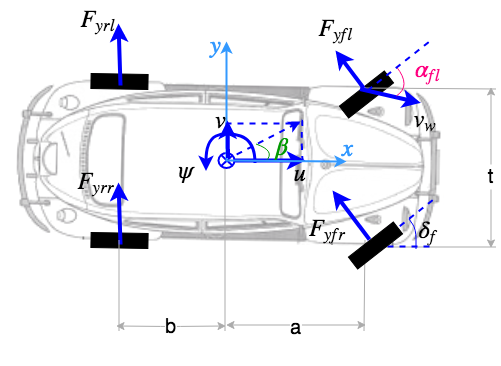
\includegraphics[width=0.7\textwidth]{carmodel.png}%
\end{frame}%


%%%%%%%%%%%%%%%%%%%%%%%%%%%%%%%%%%%%%%%%%%%%%%%%%%%%%%%%%%%%%%%%%%%%%%%%
 \begin{frame}[t]%

 \noindent\textbf{Modelo compacto:}
    \begin{equation*}
    \begin{split}
    x = [\beta \quad \dot\psi \quad \dot\phi \quad \phi]^T \\
	M\dot{x} = A_Mx + B_MM_u + E_M\delta_f\\
    \end{split}
    \end{equation*}
\vspace{-0.2 cm}
\noindent\textbf{Espaço de estado:} 
    \begin{equation*}
    \begin{split}
    	\dot{x} &= Ax + [B \quad E ] u \\
    	y &= x \\
   	\end{split}
    \end{equation*}
    \begin{equation*}
    \begin{split}
    	A = M^{-1}A_M  \quad B = M^{-1}B_M \quad E =  M^{-1}E_M   \\
    \end{split}
    \end{equation*}
    \begin{equation*}
    \begin{split}
    	u = [M_U \quad \delta_f]^T & &\\
    \end{split}
    \end{equation*}
    \noindent\textbf{Espaço de estado discreto obtido no Matlab com c2d:} 
    \begin{equation*}  
    \begin{split}
    	x[k] = A_dx[k-1] + B_du[k] \quad
    	y[k] = x[k] \\
    \end{split}
    \end{equation*}
    \end{frame}%

\section{Proposta}%
  \begin{frame}[t]%
	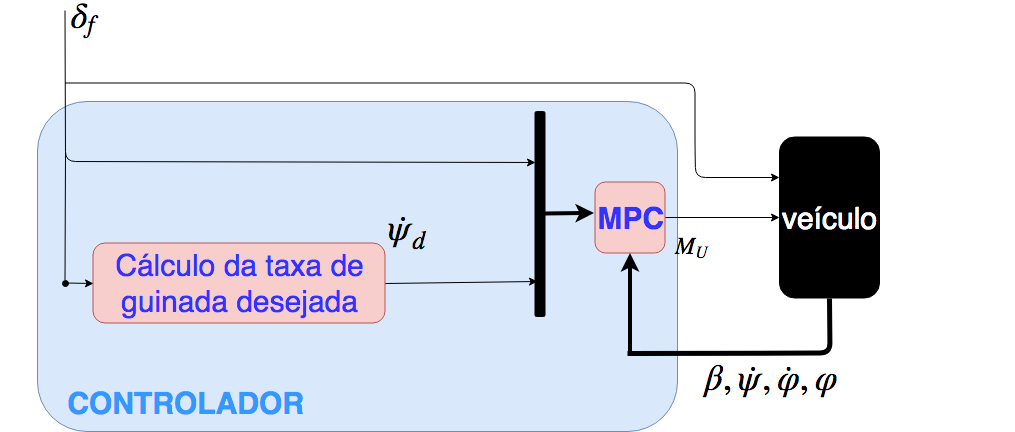
\includegraphics[width=1\paperwidth,
	height=0.5\textwidth]{BlockDiagram.png}%
	\begin{equation*}
    
    \begin{split}
    	{\dot\psi}_d = \frac{u\delta_f}{l+lK_uu^2} \\
    \end{split}
    \end{equation*}
  \end{frame}%
  

\section{Controle}%

  \begin{frame}[t]%
   	\begin{itemize}
		\item Adaptação do MPC para perturbação medida
	\end{itemize}
     
     \begin{equation*}
         \begin{split}
			x[k] &= Ax[k-1] +  B_d \begin{bmatrix} M_u[k] \\ \delta_f \end{bmatrix}\\
			B_d &= 
			\begin{bmatrix}
				B & E
			\end{bmatrix} \\
         \end{split}
     \end{equation*}
     
     \end{frame}  
     
    \begin{frame}[t]%
	
	\begin{itemize}
		\item  $Q_U \in \mathbb{R}^{2,2}$. Mas a ponderação do segundo comando é
		zero, porque ele não é controlado..
		\item O segundo comando é restrito no valor medido a priore de $\delta_f$.
	\end{itemize}
     \end{frame}   

\section{Resultados}              

  \begin{frame}%
\begin{table}[t!]
\caption{ Parâmetros do modelo utilizados na simulação}
\label{tab:model}
\begin{tabular}{|ll|ll|}
\hline
  Parâmetro     & Valor           & Parâmetro       & Valor \\
 \hline
  a             & 1.035 m          & $c_{\phi f}$     & 2823N m s/rad \\
  b             & 1.655 m          & $c_{\phi r}$     & 2652N m s/rad\\
  $t_f$         & 1.520 m          & $k_{\phi f}$     & 47298N m /rad\\
  $t_r$         & 1.540 m          & $k_{\phi r}$     & 47311N m /rad\\
  hs            & 0.451 m          & Q_U              & 1e-10  \\
  hg            & 0.550 m          & Q_Y              & diag(4,1,1e-3,1e-3) \\
  m             & 1704.7 Kg        & $I_{xz}$         & 50 $Kgm^2$   z  \\
  $m_s$         & 1526.9 Kg        & $I_{xx}$         & 744.0 $Kgm^2$ \\
  $I_{zz}$      & 3048.1 $Kgm^2$   & $C_{\alpha}$     & 90624 N/rad\\
\hline
\end{tabular}
\end{table}
   \end{frame}%
    \begin{frame}[t]%
	
	\begin{itemize}
		\item Modelo estável em malha aberta. Autovalores de $A_d$ com módulo menor do
		que 1.
	\end{itemize}
     
     Por isso desempenho esperado para o MPC foi
	\begin{itemize}
		\item Respeitando as restrições do controle fazer a taxa de guinada rastrear
		uma trajetória, mantendo o ângulo de deslizamento lateral $\beta$ e o ângulo
		de rolagem $\phi$ com módulo inferior a $\pi/18$ rad para que o sistema se
		mantenha próximo a regição de linerização, em que deve ser estável.
	\end{itemize}     
	
	Manobra simulada:
	\begin{itemize}
		\item manobra \emph{doublelane}(''mudança dupla de faixa'') a 80km/h
		em 10 segundos com esteçamento das rodas dianteiras de até $\pi/16$ rad.
	\end{itemize}     
	
     \end{frame} 

{
  \section{Resultados}%
  \begin{frame}%c
  Parametrização trivial
  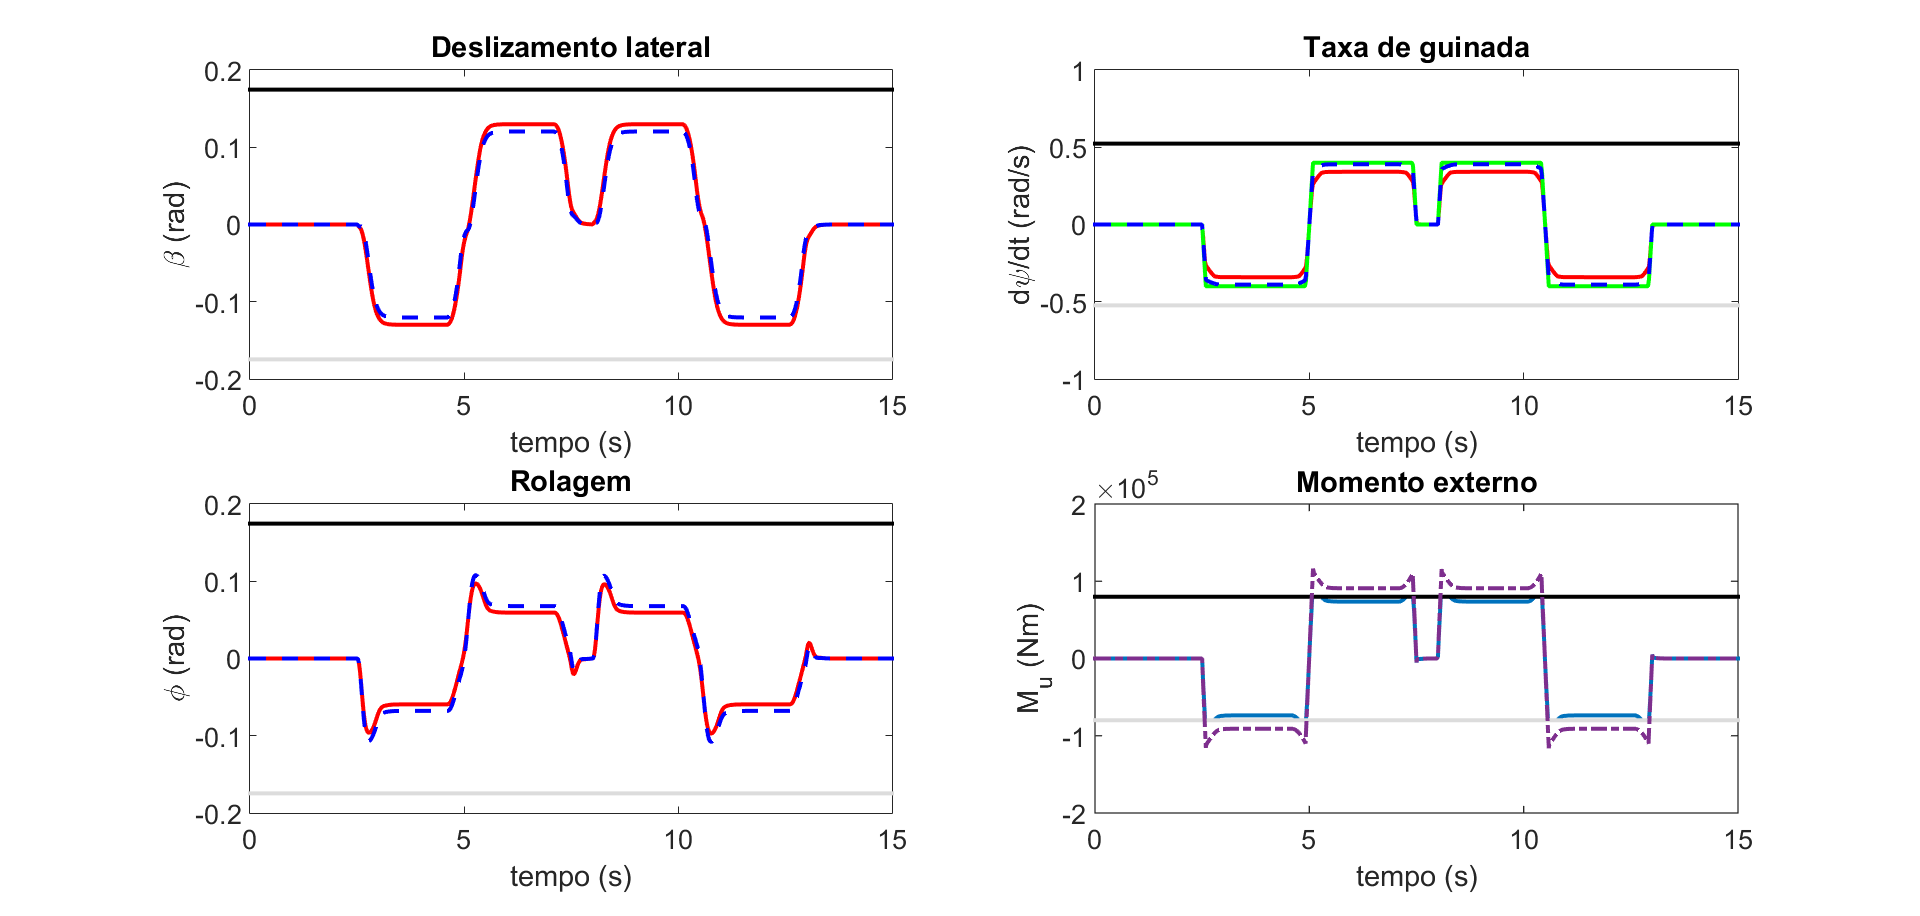
\includegraphics[width=0.8\paperwidth]{result.png}%
   \end{frame}%
      
  \begin{frame}%c
  Parametrização geral Ni = {0  50 75 };
  	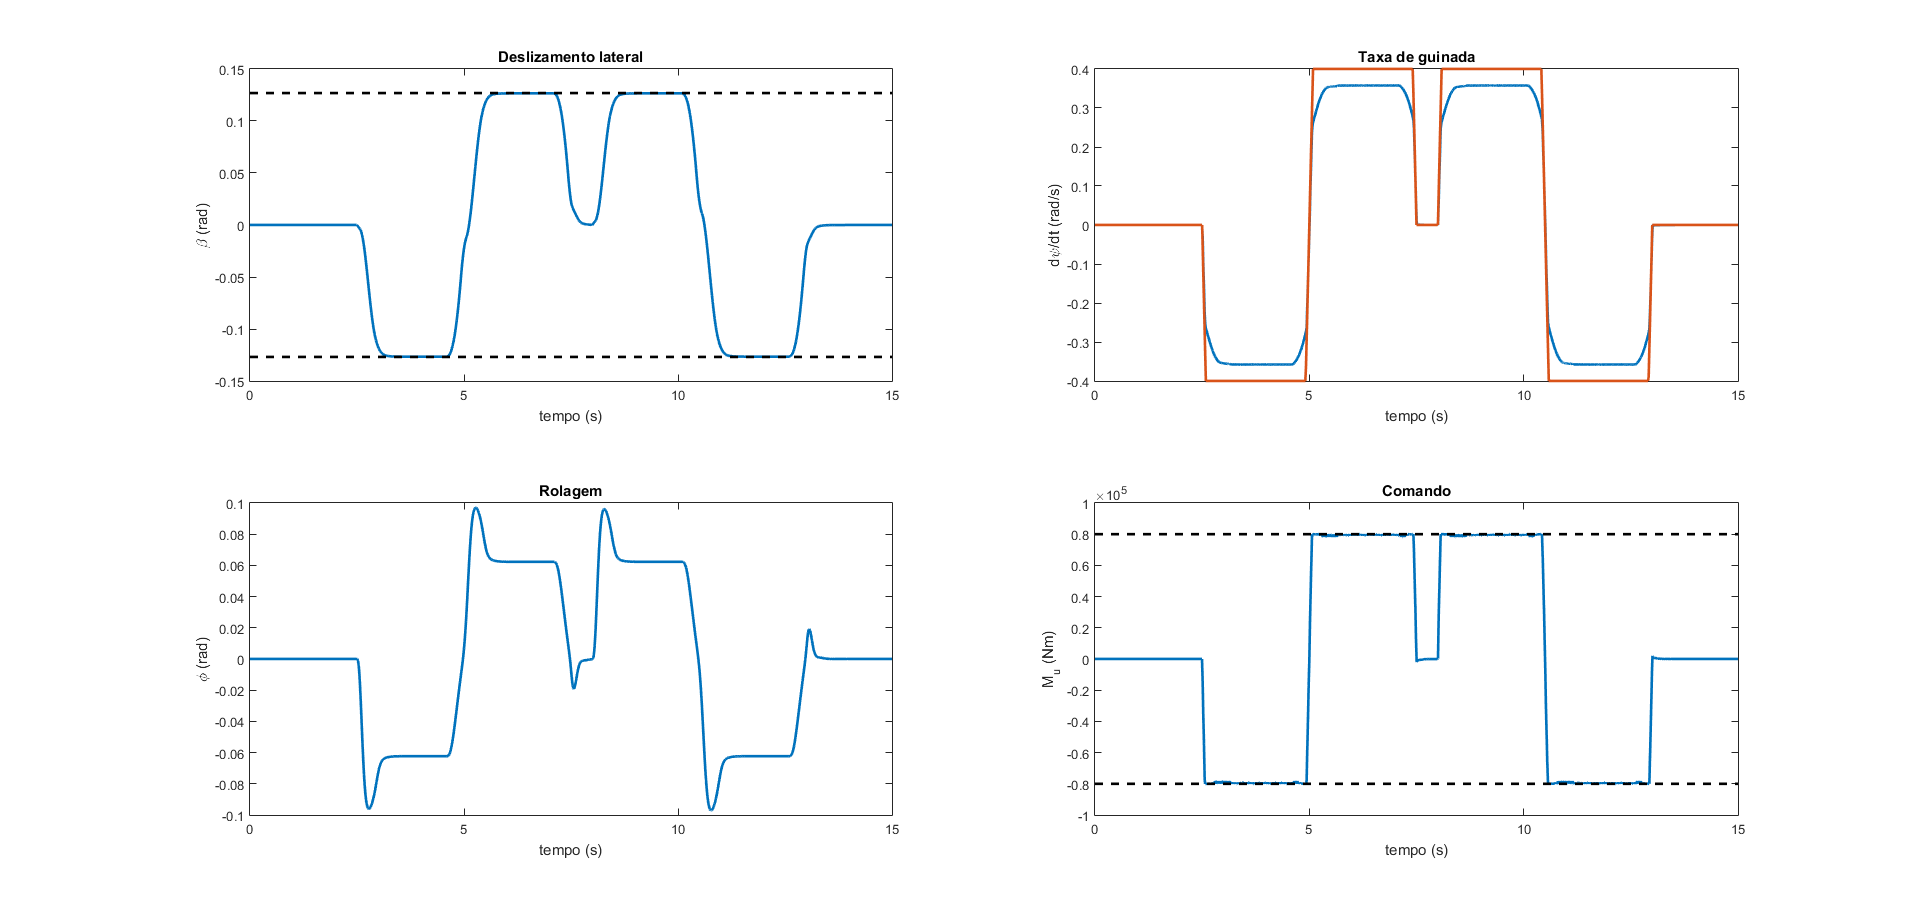
\includegraphics[width=0.8\paperwidth]{generalparam.png}%
  \end{frame}%
      
}
  
   \section{Conclusão}%
  \begin{frame}%
  	\begin{itemize}
  	\item Foi observado que com a restrição do sinal de comando, o erro da taxa
  	de guinada aumenta.
  	\item Os estados nem chegaram a alcançar o limiar da restrição. 
  	\item Quando tentou-se aplicar uma restrição aos estados, mesmo com a
  	restrição do controle em 10e20, a otimização tornou-se sem solução porque o
  	espaço de busca tornou-se vazio. 	
  	\end{itemize}
   \end{frame}%  
  
  \begin{frame}[allowframebreaks]

\bibliographystyle{IEEEtran} 
\bibliography{mylib}

\end{frame}
  
  
\end{document}
